\chapter{序論}
\section{研究の背景と目的}
AIの概念の起源は,コンピュータ開発の父,アラン・チューリング氏が1950年に提起した「機械は思考できるのか」という問いであるとされている.チューリング氏は,機械が思考したかどうかは,人との会話が成立したかどうかで判断する,とした.機械との会話が成立したかどうかの判断は次のように行う.人の審査員が,相手が見えない状況で「人」と「コンピュータ」と対話して,対話した相手が人なのかプログラムなのか言い当てる.審査員がプログラムと対話した後に「『人と』対話した」と間違った答えを出せば,「機械は思考した」ことになる.これが世にいう「チューリングテスト」である.ただチューリング氏はこのとき「AI」という言葉を使ったわけではない.チューリングテストに初めて合格したのは,2014年に発表された,ウクライナ在住の13歳の少年が開発したプログラムだった.1950年から実に64年の時間をかけてコンピュータ技術者はAIのスタートラインに立ったわけである.
\subsection{第1次AIブーム}
第1次AIブームは1950年代後半から1960年代に起きた.この時代のAIの出来事として,次の2点を紹介する. ・ダートマス会議(1956年) ・人工対話システム「エリーザ」(1964年) ダートマス会議(1956年) ダートマス会議は1956年に米ニューハンプシャー州のダートマス大学で開催された,コンピュータ研究者たちの勉強会である.いまの学会に相当する. ダートマス会議がAI史に名を残しているのは,同会議の発起人であるジョン・マッカーシー氏がAI(Artificial Intelligence,人工知能)という言葉を初めて使ったからだ.この会議で行われたデモンストレーションは,数学原理をコンピュータで証明することだった.当時のコンピュータはせいぜい四則演算が限界だったため,これは画期的な成果といえた.ただ,「コンピュータが自ら学ぶ」と理解されている現代のAIからするとまったく「AIらしくない」.人との対話チューリングテストも,到底クリアできるレベルではない. 人工対話システム「イライザ」(1966年) イライザ(ELIZA)は,マサチューセッツ工科大学(MIT)のジョセフ・ワイゼンバウム氏が1966年に作成した人工対話システムである.イライザによって人類は初めてコンピュータと会話したのである.ただイライザは「考えて回答」しているわけではなかった.例えば人がイライザに「腹が痛い」と言えば,イライザは「なぜ腹が痛いのか?」と返す.これは確かに会話だが,「からくり」があった.イライザに多数の会話パターンを仕込んでおいたのだ.よって,仕込んだパターン以外の質問をイライザにすると,イライザは回答できなくなる.しかしイライザと会話している人が偶然,ワイゼンバウム氏が想定したパターンに則した質問を続けると,見事に会話が成立した.そのため多くの人が「イライザには知性がある」と信じた. さて,第1次AIブームがしぼんだ理由は諸説あるが,最も説得的なものは「当時の技術ではブレークスルーできなかった」というものだろう.AIの理論も,AIの理論を支える技術も,そしてAIの可能性を信じてお金を出す投資家もいなかったわけである.
\subsection{第2次AIブーム}
1980年代に入り,家庭にコンピュータが普及したことにより第二次ブームが発生しました.第二次AIブームの特徴として「エキスパートシステム」が挙げられます.「エキスパートシステム」とは専門家の知識をコンピュータに教え込みことで現実の複雑な問題を人工知能に解かせることを試みたシステムです.第一次ブームと比較してコンピューターの小型化・性能が高まっており,ある程度はこれらの試みは成功しましたが,知識を教え込む作業が非常に煩雑であること,例外処理や矛盾したルールに柔軟に対応することが出来ませんでした.日常世界を見渡してみると,これらの例外処理や矛盾したルールは非常に多く,知識を教え込む作業が非常に困難なことから,第二次AIブームは自然に消滅へと向かってしまいました.その後,1990年代半ばにWindows95の登場,インターネットの普及,検索エンジンの高性能化が進み,世界中にいる誰もが簡単に大量のデータを扱える時代に突入しました.\\
\subsection{第3次AIブーム}
第二次AIブームでのエキスパートシステムが壁にぶつかった問題として,日常世界には例外処理や矛盾したルールが非常に多く,知識を教え込む作業が非常に困難というのがありました.これはコンピュータはプログラムと呼ばれるあらかじめINPUTされた命令を順次行っていくため,INPUTされていない例外処理や,矛盾したルールにぶち当たった場合に柔軟に対応出来なかったためです.これらを解決する手段として「機械学習」や「ディープラーニング」にてコンピュータが自らが学んでいくという手法が第二次AIブームの時代から研究されていましたが,実用化するためにはコンピュータの性能が追い付いていませんでした.しかし,2000年代に入り,コンピューターの小型化・性能向上に加えインターネットの普及,クラウドでの膨大なデータ管理が容易となったことで実現可能なレベルとなり,第三次AIブームが沸き起こりました.第三次AIブームでの主な出来事1997年:チェス専用のコンピューターが世界王者に勝利2006年:ディープラーニングの実用方法が登場2011年:IBMワトソンがクイズ番組で人間に勝利する2012年:画像認識の向上で画像データから「猫」を特定できるようになる2016年:「アルファ碁」がプロ棋士に勝利を収める2016年はディープラーニングを起爆剤としたAIが社会に衝撃を与え急速に発達した年であると言われています.次の年の2017年が実用的なシステムも世の中に登場し始めてきており「AI元年」と呼ばれています.このようにAIブームは1950年代の第一次AIブーム,1980年代の第二次AIブームと盛り上がっては衰退していきましたが,数々の実用的なシステムの登場により第三次AIブームは継続して続いていくだろうと予想されています.\\
\begin{figure}[!ht]
    \begin{screen}
    \begin{center}
        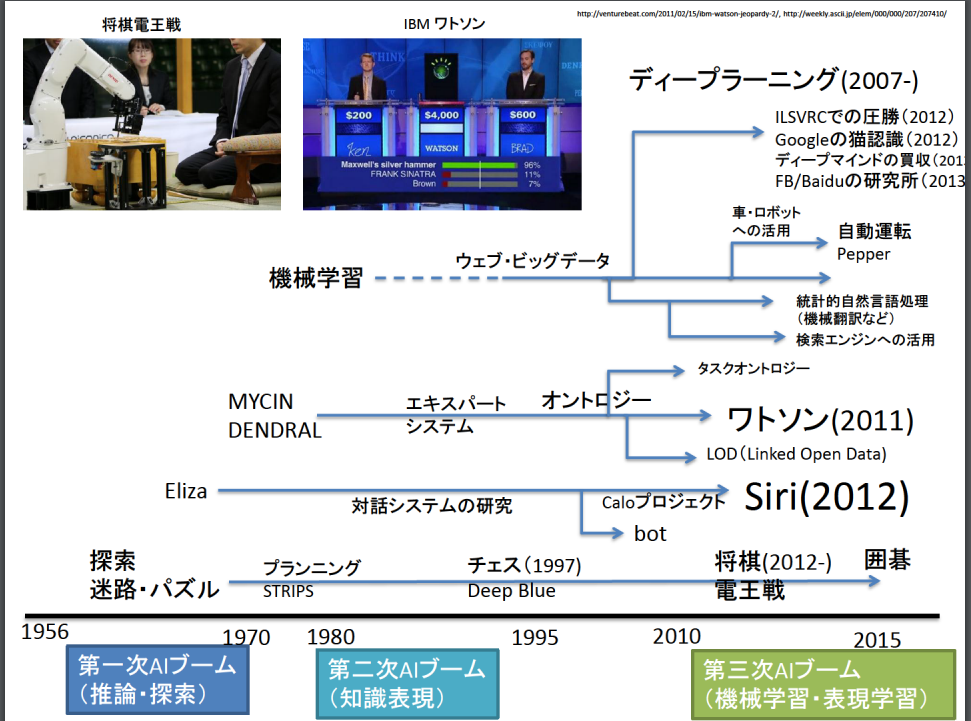
\includegraphics[scale=0.4, clip]{./img/AI_History.png}
        \caption{第一次AIブームから今までの流れ\newline(引用:https://bit.ly/2Wc9Ykb)}
        \label{fig:第一次AIブームから今までの流れ}
    \end{center}
\end{screen}
\end{figure}\\
スマートスピーカなどの対話型のAIがGoogleやAmazon,IBMによって商品化され,現在ではスマートフォンにもSiriというAIが搭載されるなどその存在は非常に身近になっており,その種類も非常に多岐にわたる.
\begin{figure}[!ht]
    \begin{screen}
    \begin{center}
        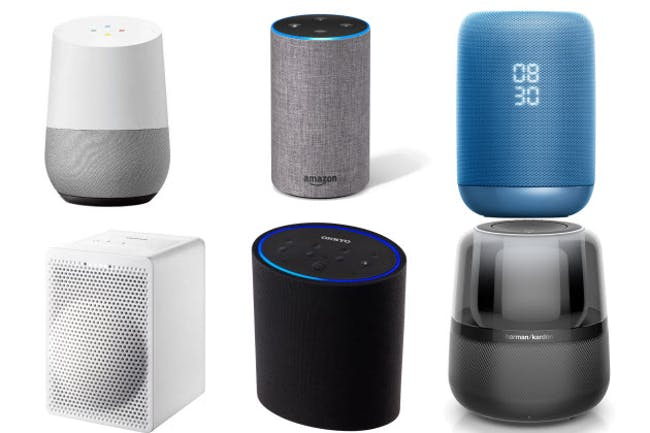
\includegraphics[scale=0.6, clip]{./img/smartspeaker_list.jpg}
        \caption{多種多様なスマートスピーカー}
        \label{fig:多種多様なスマートスピーカー}
    \end{center}
\end{screen}
\end{figure}\\
また囲碁や将棋,チェスなどの競技においても,プロにAIが勝利するなどその精度は以前から高いが,そのAIは一つの競技でしか使用できない特化型人工知能(AGI)でありった.
しかし,英DeepMindが発表したAlphaZeroという様々なボードゲームに対応できる汎用性を持ったAIが発表され,汎用人工知能(GAI)の成長も著しい.\\
自然言語処理を用いた芸術の分野では,2012年にスタートした人工知能を使って小説を生成するプロジェクトが「星新一賞」の第一審査を通過した.
また,絵画や音楽に関してもAIが作成した肖像画が米競売大手クリスティーズのオークションで43万2500ドル(約4900万円)で落札され,AIを用いて新しい作品を作るものが出回っている.\\
このようにAIの発展は様々な分野においてその成果を上げており,今後は業務の効率化や補助だけにとどまらず,自動車の自動運転や医療の現場でも人間の手よりも高精度なものとして活躍することが期待されている.
\subsection{様々なAI楽曲作成サービス}
AIを用いた楽曲作成サービスはAmper Musicという「作成したい音楽ジャンル」と「曲の長さ」を指定すれば,AIがオリジナル曲を作曲してくれるサービスです. 作成した曲は,テンポを変えたり,楽器を追加したりと後からも編集できるようにもなっている.また,Jukedeck
本研究ではAIによる楽曲生成についての実証実験を行う.
Googole brainによって公開されているTensorflowのライブラリであるMagentaはAI Duetや
そのライブラリを用いて学習データやノード数による楽曲の生成結果の違いを比較,検証し,AIによる楽曲制作が有用なものか調査する.\\
\section{本論文の構成}
本論文の構成は以下の通りである.\\
第1章では本論文の背景と目的について述べている.\\
第2章では本論文で利用する理論について述べている.\\
第3章では実験内容について述べている.\\
第4章では楽曲制作について述べている.\\
第5章ではAIを用いた楽曲制作についての本研究の結論について述べている.\\